\documentclass[conference, onecolumn]{IEEEtran} % Replace onecolumn with twocolumn if needed

% Report template for Mälardalen University
% Original template can be found: 
% https://www.overleaf.com/latex/templates/ieee-bare-demo-template-for-conferences/ypypvwjmvtdf
% Template file structure organised by: Emil Persson
% The following packages should follow the IEEE conference guidelines.

% Swedish language package 
\usepackage[utf8]{inputenc}
\usepackage[T1]{fontenc}
\usepackage[swedish,english]{babel}

% Graphics
\usepackage{graphicx, float, subfigure, blindtext}

\newcommand\IEEEhyperrefsetup{
bookmarks=true,bookmarksnumbered=true,%
colorlinks=true,linkcolor={black},citecolor={black},urlcolor={black}%
}

% Preferred hyperref setup, Michael Shell
\usepackage[\IEEEhyperrefsetup, pdftex]{hyperref}

% Maths
\usepackage{mathtools}

% These packages must be at the end
\usepackage[nolist,nohyperlinks]{acronym}
\usepackage{cleveref}
\graphicspath{{images/}}
% \acrodef{acronym}[short name]{full name}
\acrodef{IC}[IC]{Integrated Circuit}
% \acrodef{svm}[SVM]{Support Vector Machine}
\newacro{svm}[SVM]{Support Vector Machine}
% Example use \ac{IC} for printing "Integrated Circuit (IC), use \ac{IC} again and it will print (IC)"
% For plural use \acp{IC} for short and \aclp{IC} for long.
% For more see: http://ftp.acc.umu.se/mirror/CTAN/macros/latex/contrib/acronym/acronym.pdf

% Swedish language package 
\usepackage[utf8]{inputenc}
\usepackage[T1]{fontenc}
\usepackage[swedish,english]{babel}

% Graphics
\usepackage{graphicx, float, subfigure, blindtext}

% \newcommand\IEEEhyperrefsetup{
% bookmarks=true,bookmarksnumbered=true,%
% colorlinks=true,linkcolor={black},citecolor={black},urlcolor={black}%
% }

% Preferred hyperref setup, Michael Shell
% \usepackage[\IEEEhyperrefsetup, pdftex]{hyperref}

% Maths
\usepackage{mathtools}

% These packages must be at the end
\usepackage[nolist,nohyperlinks]{acronym}
\usepackage{cleveref}
\graphicspath{{images/}}

% Remove section first paragraph indent
\usepackage{titlesec}
\titlespacing*{\section}{0pt}{*1}{*1}
\titlespacing*{\subsection}{0pt}{*1}{*1}
\renewcommand{\thesubsubsection}{\arabic{subsubsection}}
\titleformat{\subsubsection}[runin]{\itshape}{\thesubsubsection)}{1em}{}[:]
\titlespacing*{\subsubsection}{\parindent}{0pt}{*1}

% Include authors
\author{\IEEEauthorblockN{
Carl-Johan Höglind\IEEEauthorrefmark{1},
Author 2\IEEEauthorrefmark{2}
}

\IEEEauthorblockA{
School of Innovation, Design and Engineering\\
Mälardalen University, Västerås, Sweden\\
Email:
\IEEEauthorrefmark{1}chd16002@student.mdu.se,
\IEEEauthorrefmark{2}author2@student.mdu.se
}}

% The report title.
\title{Report Title Here\\
Mälardalen University}

% Document begins here
\begin{document}

    % Create the title.
    \maketitle
    % Example sections, name them
    % according to specific needs.
    \section{Question 1} 

    \section{Question 2}
        \subsection{a}
            Sufficient schedulability test for RM scheduling: $U <= n(2^{1/n} - 1)$ \\ where n is the number of tasks in the task set and U is the processor utilization factor, $U = \sum_{i=1}^{n} \frac{C_i}{T_i}$. 

        \renewcommand{\arraystretch}{1.4}
        \begin{figure}[H]
        \centering
        \begin{minipage}{0.5\textwidth}
            \begin{table}[H]
            \centering
            \begin{tabular}{|l|l|l|}
                \hline
                \textbf{Task}   & \textbf{T=D}  & \textbf{C}  \\ \hline
                A               & 3             & 1           \\ \hline
                B               & 5             & 2           \\ \hline
                C               & 2             & 0.5         \\ \hline

            \end{tabular}
            \end{table}
        \end{minipage}%
        \caption{Task set}
        \label{fig:Taskset}
        \end{figure}
    \renewcommand{\arraystretch}{1.0}

        \subsubsection{Task set schedulable?}
        $U = \sum_{i=1}^{n} \frac{C_i}{T_i} = \frac{1}{3} + \frac{2}{5} + \frac{0.5}{2} = 0.98$ \\
        $U <= n(2^{1/n} - 1) = 3(2^{1/3} - 1) = 0.78$ \\
        Since the statement $U <= n(2^{1/n} - 1)$ is false in this case, the task set cannot be proven to be schedulable with this sufficient test method.

        \subsection{b}
            \subsubsection{Exact schedulability test, Tracing}
            \begin{figure}[H]
                \centering
                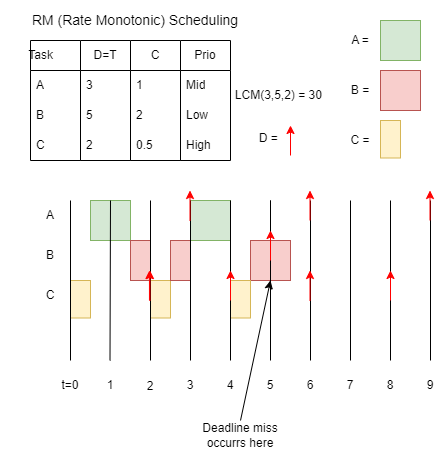
\includegraphics[width=0.5\textwidth]{images/Ass1Q2.drawio.png}
                \caption{Tracing of the task set proves that it is not schedulable with RM.}
                \label{fig:tracing}
            \end{figure}

            As demonstrated in figure \ref{fig:Taskset}, the task set is not schedulable with RM scheduling. The task set is not schedulable because task B misses its deadline at $t = 5$.

    \section{Question 3}

    To calculate the maximum execution time for Task A to make the task set schedulable, the first thing to try is to make the statement $U <= n(2^{\frac{1}{n}} - 1)$ true. In this case $n = 3$ which gives us $U <= 0.78$. So continuing from there we can find the maximum $Ca$ using the equation $U = \sum_{i=1}^{n} \frac{C_i}{T_i}$. The following table contains the given values for period and execution time for the tasks.
    \renewcommand{\arraystretch}{1.4}
        \begin{figure}[H]
        \centering
        \begin{minipage}{0.5\textwidth}
            \begin{table}[H]
            \centering
            \begin{tabular}{|l|l|l|}
                \hline
                \textbf{Task}   & \textbf{T=D}  & \textbf{C}  \\ \hline
                A               & 4             & Ca          \\ \hline
                B               & 12            & 4           \\ \hline
                C               & 20            & 9           \\ \hline
            \end{tabular}
            \end{table}
        \end{minipage}%
        \caption{Task set}
        \label{fig:Q3tasks}
        \end{figure}
    \renewcommand{\arraystretch}{1.0}

    Using the values in the table and the formula $U = \sum_{i=1}^{n} \frac{C_i}{T_i}$ we can extract $Ca$ and get the following equation: $Ca = 4*(0.78 - \frac{4}{12} - \frac{9}{20}) = -0.014ms$. This is not a valid value for $Ca$, so we need to try another approach.\\
    
    We will now try a different approach by finding the worst case execution time (WCET) for task C which is the lowest priority task according to RM scheduling protocols. WCET for task C cannot be slower than $20ms$ because then it will miss its deadline. WCET is found by releasing all higher priority tasks at the same time as task C, but since we do not know the execution time of task A we will only release task B and C and then find the remaining execution time within the $20ms$ period. Within the $20ms$ time period task B will be released twice and execute a total of $2*4ms = 8ms$, task C will be released once and execute a total of $9ms$. If we add up the execution time of task B and C we get $8ms + 9ms = 17ms$. This means that the remaining execution time for task A is a total of $20ms - 17ms = 3ms$. To find the maximum execution time for task A we will have to divide the remaining free time in the $20ms$ period with the number of times task A is released. Task A is released every $4ms$ which means that it will be released $5$ times within the $20ms$ period. The maximum execution time for task A is then $\frac{3ms}{5} = 0.6ms$. So the maximum execution time for task A is $0.6ms$ to make the task set schedulable.

    % We will now try to find maximum $Ca$ by calculating the total amount of execution time needed for all tasks in one hyperperiod. The hyperperiod, or the lowest common multiple (LCM) of the periods of the tasks, is $60ms$. We need to find how many instances occur of each task and then multiply it by the execution time of each task.\\
    % Instances of each task in one hyperperiod:
    % \begin{itemize}
    %     \item Instances of task A: $\frac{LCM}{Ta} = \frac{60}{4} = 15$
    %     \item Instances of task B: $\frac{LCM}{Tb} = \frac{60}{12} = 5$
    %     \item Instances of task C: $\frac{LCM}{Tc} = \frac{60}{20} = 3$
    % \end{itemize}
    
    % The total amount of execution time needed for all tasks in one hyperperiod is then:
    % \begin{itemize}
    %     \item Task A: $15*Ca =?$
    %     \item Task B: $4*5 = 20ms$
    %     \item Task C: $9*3 = 27ms$
    % \end{itemize}

    % We now have the following equation: $15*Ca + 20 + 27 <= 60$. Solving for $Ca$ gives us $Ca <= \frac{60-27-20}{15} = 0.87ms$. This gives us a maximum execution time for task A of $0.87ms$ to make the task set schedulable.\\

    \section{Question 4}
\label{sec:question4}
    
    \section{Question 5}

    To make a task set that is schedulable by EDF but not RM i will find a task set that gives a utilization factor $U = 1$. This will be schedulable with EDF but it is not guaranteed that it is schedulable with RM. To make a task set with $U = 1$ i will use the following equation: $U = \sum_{i=1}^{n} \frac{C_i}{T_i} = 1$. I will use the following task set: 

    \renewcommand{\arraystretch}{1.4}
        \begin{figure}[H]
        \centering
        \begin{minipage}{0.7\textwidth}
            \begin{table}[H]
            \centering
            \begin{tabular}{|l|l|l|}
                \hline
                \textbf{Task}   & \textbf{T=D}  & \textbf{C}  \\ \hline
                A               & 3             & 1           \\ \hline
                B               & 6             & 2           \\ \hline
                C               & 9             & 3           \\ \hline
            \end{tabular}
            \end{table}
        \end{minipage}%
        \caption{Task set}
        \label{fig:Q5tasks}
        \end{figure}
    \renewcommand{\arraystretch}{1.0}

    The task set in figure \ref{fig:Q5tasks} has a utilization factor of $U = \sum_{i=1}^{n} \frac{C_i}{T_i} = \frac{1}{3} + \frac{2}{6} + \frac{3}{9} = 1$. This task set is schedulable with EDF but most likely not with RM. To prove this I will draw the trace for each scheduling algorithm.\\

    \begin{figure}[H]
        \centering
        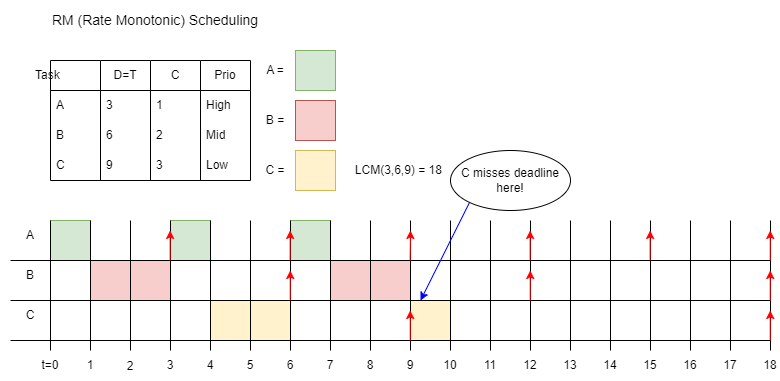
\includegraphics[width=0.8\textwidth]{images/Ass1Q5RM.png}
        \caption{Tracing of the task set with RM scheduling does not work as seen in the figure. The red arrows in the figure indicate the deadlines/period for the tasks.}
        \label{fig:Q5RMtrace}
    \end{figure}

    As seen in figure \ref{fig:Q5RMtrace} the task set is not schedulable with RM scheduling. Task C misses its deadline at $t = 9$.\\

    \begin{figure}[H]
        \centering
        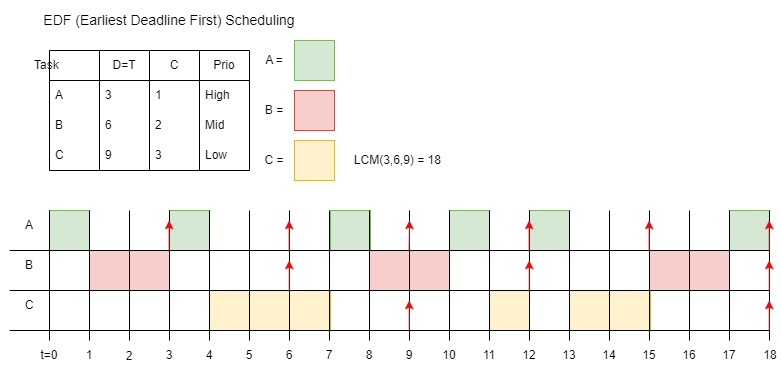
\includegraphics[width=0.8\textwidth]{images/Ass1Q5EDF.drawio.png}
        \caption{Tracing of the task set with EDF scheduling is feasable as seen in the figure. The red arrows in the figure indicate the deadlines/period for the tasks.}
        \label{fig:Q5EDFtrace}
    \end{figure}
        
    As seen in figure \ref{fig:Q5EDFtrace} the task set is schedulable with EDF scheduling. The task set is schedulable with EDF because the task with the earliest deadline is always executed first which guarantees schedulability as long as $U <= 1$.\\
    \section{Question 6}
    \section{Question 7}
    \section{Question 8}
    %\begin{abstract}
    
\end{abstract}
    %\begin{center}
    \begin{IEEEkeywords}
    Alphabetical, Be, In, Order, Should
    \end{IEEEkeywords}
    \end{center}
    %\section{Introduction}
\label{section:intro}
\blindtext

Here are a new paragraph and some examples of references and an abbreviation \cite{IEEEtran, IEEEtranformatexample, webpage, FundConDep, exampleofjournalarticle, exampleofconferencepaper}
\ac{svm}. When citing works, never start a sentence with a number. In such situations, write, e.g., "Liang et al. \cite{exampleofconferencepaper}" instead.

Generally, this section provides an introduction and literature overview, aim of the work and research questions.
    %\section{Method}
    %\section{Results}
\label{section:results}

\section{Question 1} 
        \subsection{Part 1}
            \subsubsection{Sufficient and necessary schedulability test}
            A suffiient schedulability test provide a guarantee of schedulability when passed. If the test is fulfilled, it ensures that the task set is schedulable. However if it is not passed, it does not provide any conclusive answer about schedulability. On the other hand, a necessary schedulability test provides a guarantee of unschedulability when failed. Conclusively, an exact schedulability test, which is both sufficient and necessary, can always guarantee whether the task set is schedulable or not.

            \subsubsection{Feasible schedule}
            A feasible schedule is simply a schchedule for a task set that is schedulable in a way so that all tasks completed within their deadlines. In other words, it is a schedule where all tasks meet their timing requirements without violating any system constraints.

            \subsubsection{Task and task instance}
            A task is a set of instructions that are executed within a larger program by a processor. A task instance refers to a single execution or occurrence of a task.

            \subsubsection{Task and processor utilization factor}
            The processor utilization factor is denoted by U, and is used to describe how much time of the processor is used. U is ranging from 0 to 1 or 0-100\% describing the time utilization of the processor. The processor utilization factor is calculated by dividing the total execution time by the total period time of the task set.If U is larger than 1 (or 100\%), the task set is not schedulable because the task set needs more processor time is required than is available.
            

            \subsubsection{Static and dynamic priority scheduling}
            Static priority scheduling and dynamic priority scheduling are two different approaches to online scheduling. Static priority scheduling is a scheduling method where the priority of a task is fixed and determined pre-run-time, it does not change during run-time. Dynamic priority scheduling is a scheduling method where the priority of a task is not fixed and can change during run-time. The change of the priorities in dynamic priority scheduling is based on the current state of the system.

            \subsubsection{Critical instant}
            A critical instant represents the worst-case scenario for a task in terms of meeting its deadline and timing constraints. The critical instant occurs when higher-priority tasks preempt the task in question, causing it to experience the longest possible delay before it can resume execution. If a task can meet its deadline at its critical instant, it ensures that the task will meet its timing requirements under all other conditions as well.

        \subsection{Part 2 - Offline scheduling}
            \subsubsection{Schedulability}
            Offline scheduling offers more room for complexity and predictability. This is because the execution pattern is known and it can be changed in a predictable way to make processor utilization more efficient, fit more tasks in the task set etc. The schedulability is provable by construction since it will always execute the task set in the same way and can therefore be analyzed and verified before run-time.

            \subsubsection{Predictability}
            Offline scheduling is more predictable than online scheduling since the schedule is constructed before run-time. This means that the system will behave the exact way it was designed, unless some external factors affect the system e.g. hardware failure etc.

            \subsubsection{Flexibility}
            In offline scheduling, the schedule is predetermined and does not change once the system begins operating. This means that the system is not flexible and cannot adapt to changes in the environment or system.

            \subsubsection{Communication and synchronization}
            Communication refers to the exchange of data between tasks or components. 

            \subsubsection{Jitter}
            Jitter is the variation in the execution time of a task. It is the difference between the best-case execution time and the worst-case execution time. A system with low jitter is more predictable than a system with high jitter.

            \subsubsection{Heuristic}
            If we are traversing a search tree, we can use heuristic strategy to choose which branch to traverse in the tree. We can choose for example to go with the task that has the earliest deadline, or the task with the shortest execution time etc. Heuristic is a way to make a decision based on some criteria, without knowing the exact outcome of the decision. 


    \section{Question 2}
        \subsection{a}
            Sufficient schedulability test for RM scheduling: $U <= n(2^{1/n} - 1)$ \\ where n is the number of tasks in the task set and U is the processor utilization factor, $U = \sum_{i=1}^{n} \frac{C_i}{T_i}$. 

        \renewcommand{\arraystretch}{1.4}
        \begin{figure}[H]
        \centering
        \begin{minipage}{0.5\textwidth}
            \begin{table}[H]
            \centering
            \begin{tabular}{|l|l|l|}
                \hline
                \textbf{Task}   & \textbf{T=D}  & \textbf{C}  \\ \hline
                A               & 3             & 1           \\ \hline
                B               & 5             & 2           \\ \hline
                C               & 2             & 0.5         \\ \hline

            \end{tabular}
            \end{table}
        \end{minipage}%
        \caption{Task set}
        \label{fig:Taskset}
        \end{figure}
    \renewcommand{\arraystretch}{1.0}

        \subsubsection{Task set schedulable?}
        $U = \sum_{i=1}^{n} \frac{C_i}{T_i} = \frac{1}{3} + \frac{2}{5} + \frac{0.5}{2} = 0.833$ \\
        $U <= n(2^{1/n} - 1) = 3(2^{1/3} - 1) = 0.7798$ \\
        Since $U > n(2^{1/n} - 1)$, the task set is not schedulable.

        \subsubsection{Task set schedulable with RM?}
        The task set is not schedulable with RM since the processor utilization factor is larger than the threshold for RM scheduling. 

        \subsubsection{Task set schedulable with EDF?}
        The task set is not schedulable with EDF since the processor utilization factor is larger than the threshold for EDF

% \begin{figure}[H]
%     \centering
%     \subfigure[MDH logo]{
%     \label{fig:MDH1}
%     
\includegraphics[width=.2\columnwidth]{MDHlogga}}
%     \qquad
%     \subfigure[MDH logo]{
%     \label{fig:MDH2}
%     
\includegraphics[width=.2\columnwidth]{MDHlogga}}
%     \qquad
%     \subfigure[MDH logo]{
%     \label{fig:MDH3}
%     
\includegraphics[width=.2\columnwidth]{MDHlogga}}
%     \caption[Short text]{This is a example of multiple figures.}
%     \label{fig:MDHlogga}
% \end{figure}
    %\section{Discussion}\label{section:disc}
    
    %\section{Conclusion}
\blindtext
    %\section*{Acknowledgment}
The authors would like to thank ... for his/her/their help and support during the process of writing this paper. 
    % Select the IEEEtran style
    %\bibliographystyle{IEEEtran}
    % Include bibliography file
    %\bibliography{IEEEabrv, refs}

\end{document}